Модели Эло служат для оценки способностей,но не исследуют проблему оптимального уровня сложности.
Заметим, что значения в пределах интервала 2 сигма от текущего рейтинга статзначимо различимы лишь $5\%$ экспериментов. 

Тогда естественным разделением по сложности является:

\begin{figure}[h]
    \centering
    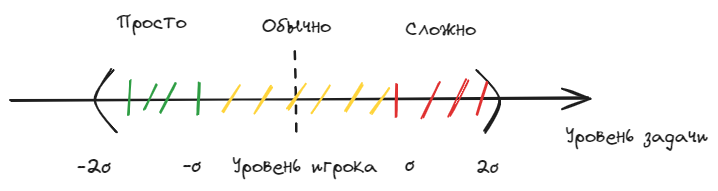
\includegraphics[width=0.5\textwidth]{assets/work/rating/interval.excalidraw.png}
    \caption{Разделение сложности на естественные интервалы}
    \label{interval}
\end{figure}

Таким образом задача ассистента, исходя из ответов пользователя задавать промежуток. Текущая работа также предлагает учесть время исполнения занятия. Для этого введем симплекс $S$, ограниченном разницей сложности не более чем 2 стандартных отклонения.

Уровень сложности будем определять как случайную величину $\xi$, равномерно распределенную на предложенном симплексе $s = \left[0,\infty\right] \times \left(-2\sigma,2\sigma\right)$.

Тогда генерация новой задачи будет выполняться путем генерации из равномерного распределения $\xi \sim U(S)$

\begin{figure}[h]
    \centering
    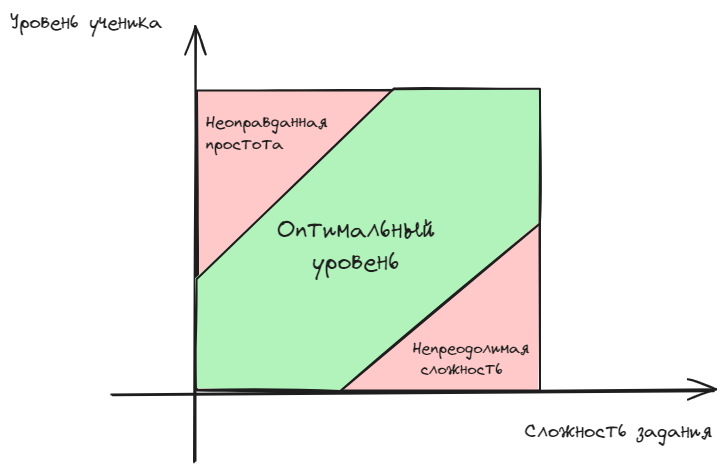
\includegraphics[width=0.5\textwidth]{assets/work/rating/restricted.excalidraw.png}
    \caption{Ограничение области сложности естественным}
    \label{restrict}
\end{figure}

\texit{Стохастическая аппроксимация}


Для решения задачи был предложен алгоритм Роббинса Манро \cite{robbins1951stochastic}.


$$
    \theta_1 = \theta_n - a_n \left(N(\theta_n) -\alpha\right)
$$



По форме метод похож на метод Ньютона




В основе подхода 

Подобный подход широко используется в игровой индустрии и направлен на создание психологического состояния потока, описанного в работе \cite{csikszentmihalyi2005flow}

Таким образом мы исключим задачи не соответствующие текущему уровню игрока и обеспечим разнообразие в постановках задач. 

Альтернативный подход к адаптивному 
пересчету сложности описан в работе \cite{yazidi2020balanced}.
Авторы предполагают наличие функции $S(d)$ и желаемого уровня сложности.

Введем уровень сложности $d$ - как вероятность обучающегося решить задачу. Тогда прелложенную систему тестирования можно представить
как многошаговая система c нумераций $t$, на каждом этапе которой сложность задачи $d(t+1)$ определяется 
исходя из результата $x(t)$ решения по правилу

$$
    d(t+1) = \begin{array}
        \min{1,d(t)+\lambda (1-s)} \\
        \max{0,d(t) - \lambda s} \\
    \end{array} 
$$

, где $\lambda$ - параметр адаптации.

Случайный процесс соотвествует методу cтохастической аппроксимации.
Приведем ключевые теоремы, изучающие сходимость предложенной системы.


\textit{Теорема} Стохастический процесс $d(t)$ сходится к одному из трех случаев при $\lambda \rightarrow 0$ \begin{itemize}
    \item для $<s>$
\end{itemize}
\textit{Доказательство}\qed
Для доказательства используем \cite{harold1997stochastic}

\blacksquare


Альтернативным путем является подход байесовской оценки знания,
описанный в работе \cite{corbett1994knowledge}


\begin{figure}[h]
    \centering
    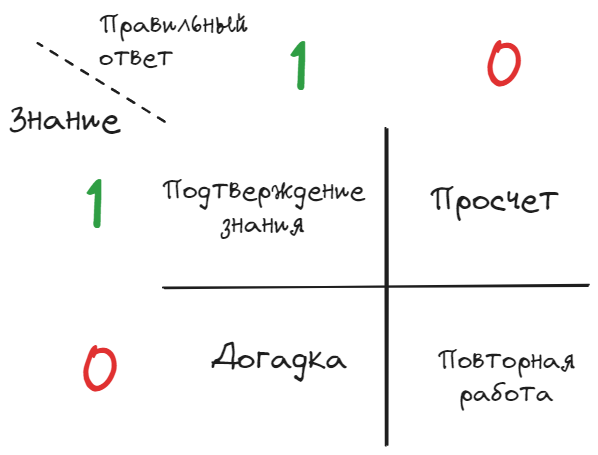
\includegraphics[width=0.5\textwidth]{assets/work/rating/bkt.excalidraw.png}
    \caption{Матрица исходов модели Байесовской оценки на шаге t}
    \label{bkt}
\end{figure}

Задача модели подобрать три ключевых параметра \begin{itemize}
    \item $P(L_0)$ начальные знания в предмете
    \item $P(S) = P(x=0| L_t = 1)$ вероятность просчета при наличи знаний
    \item  $P(G) = P(x=1| L_t = 1)$ вероятность угадать при отсутствии знаний
\end{itemize}

При их подборе Байесов подход к оценке
позволяет обновлять представления о
степени знаний согласно правилам

$$  
    P(L_t| obs_t=1) = \frac{P(L_t)(1-P(S)}{P(L_t)(1-P(S)) + (1-P(L_t))P(G))} \\
    P(L_t| obs_t=0) = \frac{P(L_t)P(S)}{P(L_t)(1-P(S)) + (1-P(L_t))P(G))} 
$$

\textit{Лемма} Доказательства вида апостериорного
 пересчета.
\textit{Доказательство}\qed
Сопряженным к биномальному множеству
является бета распределение 

Модель предполагает, что вероятность забыть $ P(L_{t+1}=0|L_t=1)=0$

\blacksquare

Выбор гиперпараметров выполняется с помощью EM метода.







Открытая реализация на языке Python описана в статье \cite{badrinath2021pybkt}.




